
A estrutura de dados utilizada é a VDB, renomeada para OpenVDB\footnote{www.openvdb.org} na ocasião em que foi disponibilizada com código fonte aberto. OpenVDB é uma biblioteca que inclui uma estrutura de dados compacta e hierárquica e um conjunto de ferramentas para a manipulação eficiente de dados volumétricos discretizados esparsos, que podem variar com o tempo, em um grid tridimensional. \\

A estrutura de dados foi desenvolvida pela DreamWorks Animation, e oferece um espaço de índices de três dimensões virtualmente infinito, armazenamento compacto, tanto na memória quanto em disco, acesso rápido aos dados, tanto sequencial quanto aleatório, e uma coleção de algoritmos otimizados especificamente para esta estrutura de dados para tarefas usuais como a aplicação de filtros, discretização de equações diferenciais parciais, conversão de polígonos em voxels, e amostragem. Os detalhes técnicos da estrutura de dados e de sua manipulação são discutidos nas seções seguintes.

\section{Definição}
A biblioteca OpenVDB é composta pela estrutura de dados e pelo conjunto de ferramentas para a manipulação da estrutura. Muito embora haja grande interdepeência entre estes dois itens, abordaremos cada item separadamente.

\subsection{A Estrutura de Dados VDB}
\label{vdb_data}

Uma das principais idéias em que a VDB se baseia é em organizar dinamicamente os blocos de dados de um grid em uma estrutura de dados hierárquica semelhante a uma árvore B+. Essa semelhança será abordada na seção \ref{bplus_trees}. Estes blocos são folhas\footnote{{\bf Folhas}, ou nó-folha, são os nós de uma estrutura de árvore que não possui filhos e que assim diferem da raiz e dos nós internos.} que sempre ficam em uma mesma profundidade de um grafo conectado e acíclico com fatores grandes, e variáveis, de ramificação, sendo que os fatores de ramificação são necessariamente potências de dois. Isso implica que a árvore é balanceada em altura por construção, mas baixa e larga. Como resultado, temos um domínio mais amplo, e devido à altura baixa da árvore, o número de operações de E/S necessárias para percorrer a árvore da raiz até uma das folhas é menor. \\

Templates C++ são usados frequentemente na construção da estrutura, bem como funções inline, e funções virtuais são evitadas a todo custo. Trata-se de um pequeno conjunto de otimizações que, entre outras coisas, viabiliza o acesso aleatório rápido. Mais especificamente, as classes que implementam os diferentes nós da árvore são recursivamente geradas a partir de templates em função do tipo armazenado pelos nós-filho, ao invés de usar herança de uma classe base comum a todos os nós. A motivação para esta escolha é o fato de que os nós gerados a partir de templates são expandidos inline durante a compilação, e com isso, as funções não possuem um overhead de execução, que ocorreria se a opção pelo uso de herança fosse feita.

Além disso, ao usarmos templates, fica mais fácil mudarmos a configuração de profundidade e ramificação da árvore, apesar de a escolha destas características precisar ser feita em momento de compilação, e não de execução. \\

Outras técnicas de implementação que contribuem ao desempenho da estrutura são operações bit a bit, que são muito rápidas, armazenamento de informações usando bits, uso do recurso de \texttt{union} do C++ para reuso de memória, e uso de execução paralela com suporte explícito a {\it threads} e operações SIMD\footnote{{\bf Single instruction, multiple data}, única instrução, dados múltiplos, em inglês, é uma classe de computadores paralelos na taxonomia de Flynn. Refere-se ao suporte de operações em que uma instrução é executada paralelamente em vários elementos de dados simultaneamente.}.

\subsubsection{Detalhes de implementação}
A VDB modela um espaço de índices $(x, y, z)$ infinito, embora na prática este seja limitado pela precisão de bits da arquitetura e da memória disponível. Os dados armazenados na estrutura consistem em um tipo \texttt{Valor}, definido com o uso de \texttt{templates}, e em uma coordenada com os índices discretos $(x, y, z)$, especificando a localização espacial do ponto amostral, isto é, a {\it topologia} do {\it valor} dentro da estrutura da árvore. Conforme comentado anteriormente, a menor unidade de um elemento de volume será sempre chamada de {\it voxel}. Um único {\it valor} é associado a cada voxel. E cada voxel pode existir em um de dois estados possíveis - são eles: {\it ativo} e {\it inativo}. A interpretação deste estado binário depende da aplicação que estiver usando a biblioteca, mas podemos considerar que os voxels ativos são mais importantes, ou de maior interesse, para a aplicação. \\

A VDB armazena separadamente a {\it topologia} de um voxel numa árvore cujo nó raiz cobre todo o espaço de índices e cujas folhas cobrem um subconjunto fixo do espaço de índices. Mais precisamente, a topologia é armazenada implicitamente em máscaras de bit, e os valores associados a cada voxel são armazenados de maneira explícita em buffers que podem estar localizados em qualquer nível da árvore - dizemos que a estrutura é multiníveis por isso. Áreas do espaço de índices em que todos os voxels tem o mesmo valor podem ser representados com uma única entrada no nível correto da árvore. Assim como voxels, os valores armazenados nos níveis intermediários da árvore também podem estar ativos ou inativos. O objetivo da VDB é usar o mínimo de memória possível para representar os voxels ativos, mantendo as características de desempenho de uma estrutura de dados para volumes densos. \\

Um componente fundamental da estrutura de dados é o conjunto de máscaras de bit incluídas nos vários nós da árvore, em diferentes níveis. O uso das máscaras de bit permitem acesso rápido e direto à representação binária da {\it topologia} local ao nó.  Um diagrama mostrando a estrutura interna da VDB é apresentado na Figura \ref{treeStructure}. \\

%figura aqui!! :-P
\begin{figure}[!htb]
\center
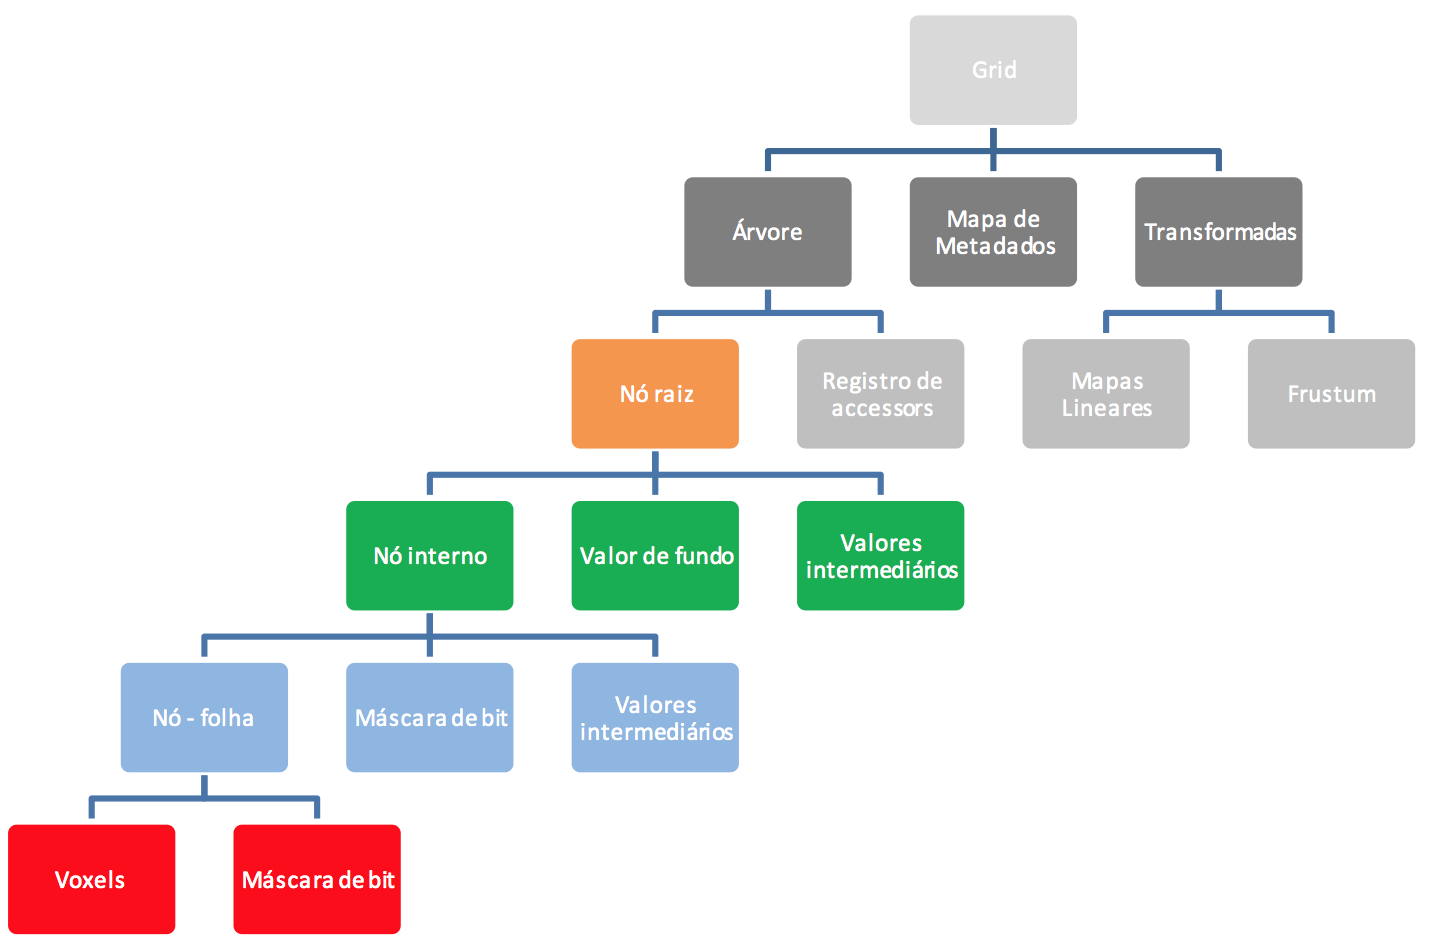
\includegraphics[width=16cm]{tree_structure}
\caption{Diagrama da estrutura interna da árvore VDB.}
\label{treeStructure}
\end{figure}

{\emph Folhas}. Estes nós são os blocos do grid de nível mais baixo na estrutura, e por construção, todos estão na mesma profundidade da árvore.As folhas dividem o espaço de índices em subdomínios disjuntos com $2^{log(2w)}$ voxels em cada eixo, onde $2^{log(2w)} = 1, 2, 3, ...$ e $w$ é qualquer entre $x$, $y$ ou $z$. Uma configuração típica, e recomendada, é estabelecer $2^{log(2w)} = 3$, o que corresponde a um bloco $8 \times 8 \times 8$. As dimensões das folhas (e dos nós internos, que discutiremos a seguir) são restritas a potências de dois, pois isso permite as operações bit a bit com mais velocidade durante as buscas pela árvore.

\lstinputlisting[label=leafNode,caption=Definição de um nó folha.]{sourceCode/leafNode.cpp}

Como pode ser visto no Código \ref{leafNode}, os tamanhos são estabelecidos em momento de compilação, e o tamanho do nó é computado como $1 << \sum_{w} sLog2w$, onde $<<$ denota um deslocamento de bits à esquerda. As folhas armazenam os valores dos voxels em uma tabela chamada de {\it Direct Access Table}\footnote{Pode-se assumir que esta tabela é um vetor com custo de acesso aleátorio de $O(1)$ para o pior caso.}, denotada no código por \texttt{mLeafDAT}, e a topologia do voxel ativo é mantido na máscara de bits denotada no código por \texttt{mValueMask}. É importante notar que embora a máscara de bits tenha um tamanho fixo igual ao da estrutura \texttt{LeafNode}, o tamanho do vetor que armazena os valores dos dados é dinâmico, mantido em \texttt{mLeafDAT.values}. A quantidade variável de buffers de dados, e seus tamanhos, bem como outras informações a respeito da \texttt{LeafNode} é armazenada de forma compacta na varíavel de 64 bits \texttt{mFlags}, mostrado na Figura \ref{mFlags}.

%figura aqui!! :-P
\begin{figure}[!htb]
\center
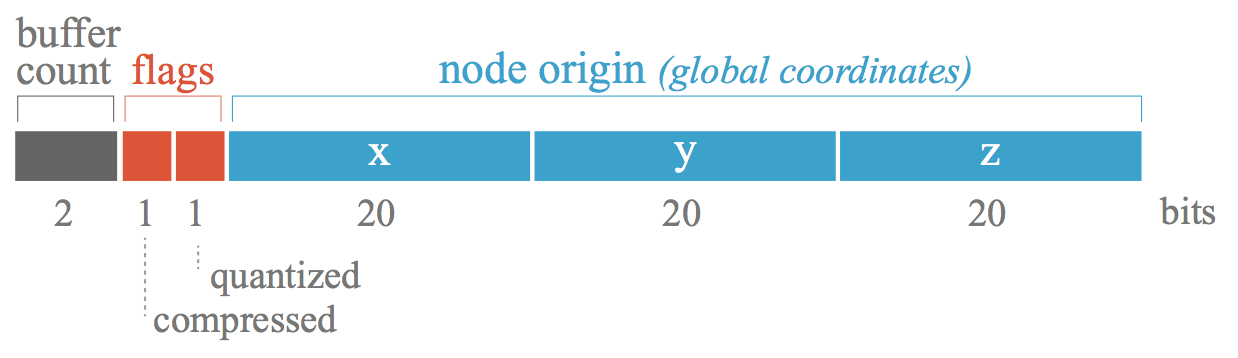
\includegraphics[width=12cm]{mFlags}
\caption{Representação compacta de \texttt{mFlags}, variável de 64 bits que codifica: número de buffers(2), compressão(1), quantização(1) e origem da folha ($3 \times 20$).}
\label{mFlags}
\end{figure}

Os primeiros dois bits codificam um dos quatro estados possíveis: 0 buffers, isto é, os valores são salvos externamente, 1 buffer, valores salvos na memória sem suporte para integração temporal, 2 buffers, valores salvos na memória com suporte a integração temporal de primeira e segunda ordem ou 3 buffers, valores salvos na memória com suporte a integração temporal de terceira ordem. O terceiro bit é 1 se o bloco é comprimido, e o quarto bit é 1 se se a folha é quantizada. Finalmente, os $3 \times 20$ bits restantes são usados para armazenar a origem do nó no grid. As coordenadas globais do voxel podem ser obtidas ao combinar a topologia local do voxel salva em \texttt{mValueMask} com a origem salva em \texttt{mFlags}. Dessa forma, as folhas são auto-suficientes e não precisam de referências para os nós pai. \\

\emph{Nós internos}. São os nós existentes em todos os níveis intermediários da árvore entre a raiz e as folhas, e basicamente definem a profundidade e o formato da árvore B+ modificada.  

\lstinputlisting[label=internalNode,caption=Definição de um nó intermediário.]{sourceCode/internalNode.cpp}

Vários detalhes da implementação são iguais aos da folha. Os fatores de ramificação são configuráveis através dos parâmetros de \texttt{template}, $Log(2w)$, e são limitados a potências de dois para buscas eficientes na árvore. Mas diferentemente das folhas, os nós internos armazenam tanto valores quanto informações de topologia, isto é, ponteiros para outros nós, internos ou folhas. A implementação é feita com o uso de \texttt{union} na tabela de acesso direto \texttt{mInternalDAT}. A topologia correspondente é armazenada de forma compacta na máscara de bits \texttt{mChildMask}, e \texttt{mValueMask} é usada para indicar se o valor intermediário está ativo ou não. Como os fatores de ramificação $Log(2w)$ são fixados na compilação, os tamanhos de \texttt{mInternalDAT}, \texttt{mChildMask} e \texttt{mValueMask} também são. Outra observação importante é que nós internos em níveis diferentes da árvore podem ter fatores de ramificação diferentes. \\

\emph{Nó raiz}. Este é o nó no nível mais alto da árvore, onde as operações sobre a árvore normalmente começam. 

\lstinputlisting[label=rootNode,caption=Definição do nó raiz.]{sourceCode/root.cpp}

Todas as configurações de uma VDB possuem no máximo um nó raiz que, diferentemente dos outros nós, é esparso e pode ter seu tamanho alterado dinamicamente. Isso é facilitado por uma tabela hash-map que armazena os ponteiros para os nós filhos ou para os valores intermediários, se forem armazenados neste nível. Se uma entrada na tabela representar um valor intermediário (como no caso de \texttt{child=NULL}), um valor booleano indica o estado do valor intermediário (se está ativo ou inativo). É importante notar que por construção o \texttt{mRootMap} contém poucos valores devido aos domínios imensos representados pelos nós intermediários, como por exemplo, $4096^{3}$.
A raiz possui um registro de classes de acesso denominada \texttt{Accessors}, que melhora consideravelmente o desempenho de acesso ao grid nos casos de consultas espacialmente coerentes ao reutilizar ponteiros de nós salvos no cache na ocasião de um acesso anterior e com isso consegue realizar a busca de baixo para cima, ao invés de percorrer a árvore de cima para baixo. \texttt{mBackground} é o valor que é retornado quando é feita uma tentativa de acesso a um local que não pertence a nenhum valor intermediário e a nenhum voxel. Uma ilustração da estrutura é apresentada na Figura

%figura aqui!! :-P
\begin{figure}[!htb]
\center
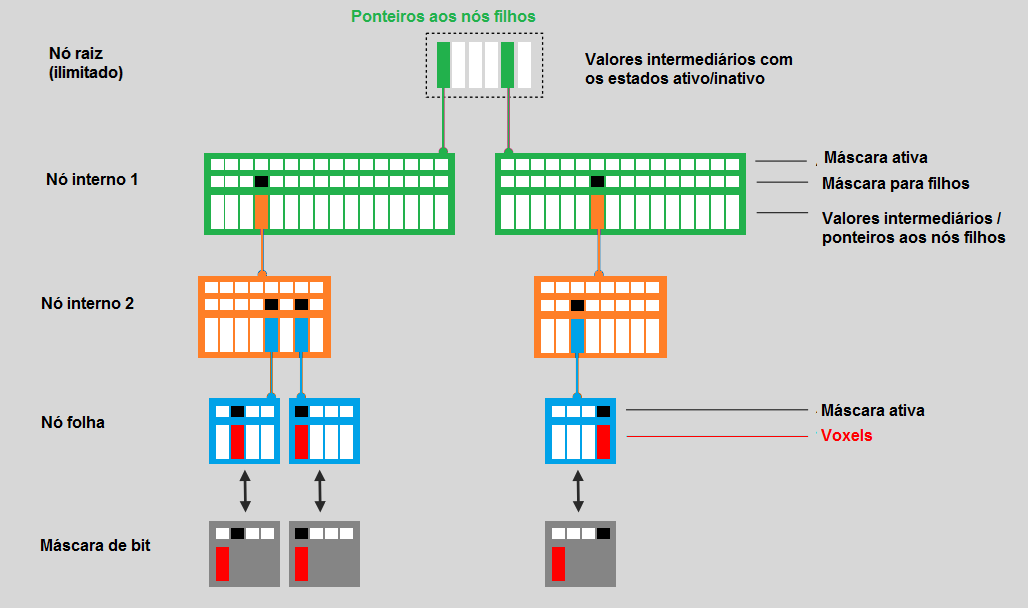
\includegraphics[width=15cm]{tree_inverted}
\caption{Ilustração unidimensional de uma VDB com um nó raiz, dois níveis de nós internos, e folhas. A raiz é dinâmica e esparsa, ao passo que os outros nós são densos e possuem fatores de ramificação que diminuem de cima para baixo, e que são restritos a potências de dois.}
\label{vdbtree}
\end{figure}


\subsection{Algoritmos de Acesso à Estrutura}
São três os tipos de acesso a uma estrutura de dados espacial: aleatório, sequencial e por estêncil. A implementação de cada uma destas formas de acesso será discutida em seguida.

\subsubsection{Acesso aleatório}
O tipo de acesso mais fundamental, e discutivelmente o de mais difícil implementação, é o acesso aleatório a voxels arbitrários. O que separa este tipo de acesso dos demais é que, no pior caso, cada acesso requer que árvore seja percorrida por inteira, de cima para baixo, começando na raiz e possivelmente terminando numa folha. Na prática, no entanto, o acesso aleatório pode ser melhorado se a ordem de busca na árvore for invertida. Deste modo, é mais fácil definir o acesso aleatório em função dos demais tipos de acesso: acesso aleatório é o tipo de acesso que não é sequencial e não é baseado em estêncis. Estes dois últimos tipos de acesso são facilmente definidos como acesso com um padrão fixo, definido pela organização dos dados na memória ou algum padrão de estêncil. \\

Como a VDB é balanceada em altura por construção com uma profundidade imutável durante a execução, todo caminho entre a raiz \texttt{RootNode} até qualquer uma das folhas \texttt{LeafNode} é igualmente longo e podemos concluir que que toda consulta aleatória leva o mesmo tempo de pior caso. Acesso aleatório a valores intermediários armazenados em níveis mais rasos da árvore é mais rápido já que a busca se encerra antes. \\

\emph{Inserção aleatória} é normalmente usada quando os grids estão sendo inicializados, mas pode ser importante também para dados dinâmicos e simulações. A busca na árvore é feita como discutido anteriormente, mas agora um nó é alocado se o bit correspondente não estiver setado em alguma \texttt{mChildMask}. A busca termina em uma folha, possivelmente recém-construída, com o valor do voxel atribuído no buffer apropriado e o bit correspondente setado em \texttt{mValueMask}. Como os nós abaixo da raiz \texttt{RootNode} são alocados apenas na inserção, o consumo de memória para dados volumétricos esparsos é baixo. E embora esta alocação dinâmica de nós implique que a inserção aleatória seja mais lenta que a consulta aleatória, o {\it overhead} é tipicamente amortizado após várias operações de inserção com coerência espacial. \\

\emph{Remoção aleatória} é outro exemplo de uma operação que requer eficiência quando lidamos com dados dinâmicos. A busca é implementada de maneira semelhante à inserção, mas agora os bits na \texttt{mChildMask} e na \texttt{mValueMask} são desmarcados e os nós são removidos se não possuírem outros filhos ou outros nós ativos. \\

Finalmente, concluímos que a VDB suporta operações aleatórias como consulta, inserção e remoção em tempo constante e isso é, na média, independente da topologia ou resolução do conjunto de dados que estão sendo armazenados.
 
\subsubsection{Acesso sequencial}
Muitos algoritmos acessam ou modificam todos os voxels ativos em um grid, mas não dependem da sequência em que isso acontece. Em particular, isso é verdade para a maioria das simulações dependentes do tempo, como advecção de fluidos. Esta invariância pode ser explorada se um padrão de acesso sequencial puder ser definido que tenha um desempenho superior àquele do acesso aleatório. \emph{Acesso sequencial}, portanto, é como nos referimos à sequência ótima de acesso aos dados, dada pela ordem em que os dados estão fisicamente dispostos na memória. Com os avanços em hierarquias sofisticadas de cache e algoritmos de pré-captura de instruções ({\it prefetching}) em CPUs modernos, torna-se especialmente importante obter e processar os dados na ordem em que estão armazenados na memória. \\

O desafio é implementar o acesso sequencial de modo que ele seja mais rápido que o acesso aleatório rápido discutido na seção anterior. O problema se resume a localizar o próximo valor ativo ou nó-filho, e a solução é bastante simples: percorrer as máscaras compactas de acesso direto \texttt{mChildMask} e \texttt{mValueMask} em cada nó. Como são estruturas compactas, são facilmente salvos em cache, e várias entradas (bits) podem ser processados simultaneamente. Como as máscaras de bit estão em todos os nós de uma árvore VDB, podemos combinar iteradores em vários níveis da árvore, permitindo a criação de iteradores que percorrem valores de voxels, valores internos ativos, folhas, entre outras possibilidades.

\subsubsection{Acesso por Estêncil}
Acesso eficiente por estêncil em grids uniformes é um requisito fundamental para cálculos de diferença finita. Esses métodos aproximam operadores diferenciais com diferenças discretas de valores em um grid numa vizinhaça local denominada estêncil de suporte. Outras aplicações deste tipo de acesso são interpolação e aplicação de filtros com {\it kernels} de convolução de suporte local. Os tamanhos e formas destes estêncis pode variar bastante dependendo da técnica aplicada. Normalmente, estes métodos de acesso são combinados com acesso sequencial, originando os iteradores de estêncil, um conceito essencial para muitas simulações numéricas.

\section{Comparação com Estruturas Semelhantes}

\subsection{Octrees}
\label{octrees}

Uma \emph{octree} é uma estrutura de dados em árvore em que cada nó interno possui exatamente 8 nós-filho. O uso mais comum da estrutura é em computação gráfica para particionar o espaço tridimensional subdividindo-o em oito octantes, de forma recursiva, como mostrado na Figura \ref{octree}. \\

No contexto de renderização, modelagem 3D e extração de malhas, esta estrutura é amplamente utilizada. E como citado na seção \ref{vdb_data}, a VDB mantém blocos organizados dinamicamente numa estrutura hierárquica, de modo que estes blocos são folhas da estrutura de árvore e que ficam todas no mesmo nível de profundidade de um grafo acíclico e conectado, com fatores de ramificação grandes, além de variáveis em momento de compilação. Logo, a VDB é balanceada em altura por construção. Octrees, por outro lado, normalmente são árvores altas, com um fator de ramificação limitado a $2$ em cada eixo ($2^3 = 8$). 
Uma característica da octree adotada pela VDB é a capacidade de armazenar valores em nós que não são folhas, funcionando como um grid multi-nível adaptativo. 

Contudo, uma limitação da VDB é que, apesar de ser uma estrutura de dados hierárquica, ela provavelmente não é a melhor escolha para métodos de amostragem multi-resolução devido aos elevados fatores de ramificação entre os níveis da árvore, e este é um dos motivos que a VDB não substitui octrees quando uma adaptatividade ótima é desejada.

%figura aqui!! :-P
\begin{figure}[!htb]
\center
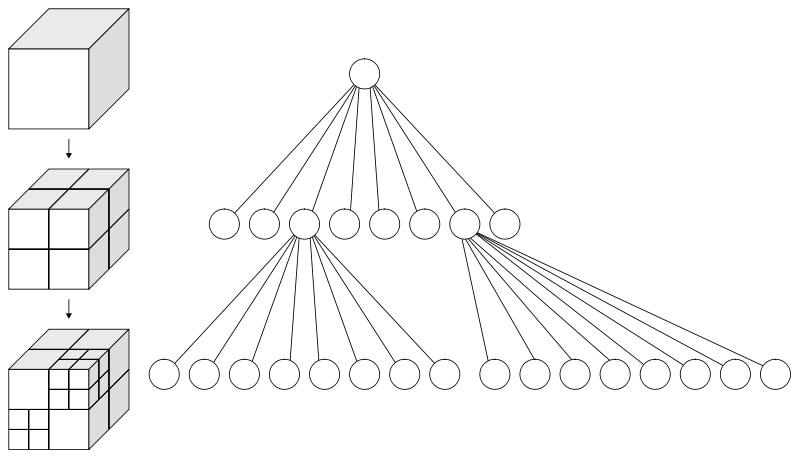
\includegraphics[width=10cm]{Octree2}
\caption{Diagrama de uma octree, estrutura em que cada nó interno possui exatamente oito nós-filho.}
\label{octree}
\end{figure}


\subsection{Árvores B}
Comentaremos brevemente acerca de árvores B para contextualizar a discussão de árvores B+, uma variação da árvore B, na seção \ref{bplus_trees}. \\

Árvore B é uma estrutura de dados que mantém os dados ordenados e permite buscas, acesso sequencial, inserções e remoções em tempo $O(log\;n)$. Trata-se de uma generalização da árvore binária de busca, sendo que esta, a árvore B, pode ter mais de dois filhos por nó. Além disso, esta árvore é otimizada para leitura e escrita de grandes volumes de dados, e por isso tem ampla aplicação em bancos de dados de sistemas de arquivos.

\subsection{Árvores B+}
\label{bplus_trees}
Uma árvore B+ é um árvore n-ária com um número variável, e normalmente grande, de filhos por nó. Uma árvore B+ consiste de raiz, nós internos e folhas. A raiz pode ser uma folha ou um nó com dois ou mais filhos.

Uma árvore B+ é uma árvore B em que cada nó que não seja uma folha possui apenas uma chave, e não pares chave-valor, com um nível a mais nas folhas. A principal aplicação de uma árvore B+ é armazenar dados para consultas rápidas em um contexto orientado a blocos de dados, como sistemas de arquivos.\\

A VDB é basicamente uma variação da árvore B+ com características de Octrees. A VDB preserva as características de desempenho das árvores B+ que resultam do uso de fatores de ramificação variáveis e grandes, mas com otimizações específicas à aplicação volumétrica. Onde, na VDB, os valores armazenados no grid são indexados por suas coordenadas espaciais em todos os nós da árvore, uma árvore B+ convencional armazena dados genéricos, isto é, de qualquer aplicação, indexados por chaves em um contexto orientado a armazenamento por blocos e somente nas folhas. Em outras palavras, VDB é uma estrutura de dados multi-nível e não usa chaves no sentido tradicional como a árvore B+ o faz. Além disso, em várias implementações as folhas de uma árvore B+ são ligadas umas às outras para permitir uma iteração sequencial rápida, diferentemente da VDB que opta por salvar em cache os caminhos de busca percorridos. Finalmente, nas árvores B+ o custo de uma busca aleatória é logarítmico, ao passo que com a VDB o custo de busca é constante. 
 
%figura aqui!! :-P
\begin{figure}[!htb]
\center
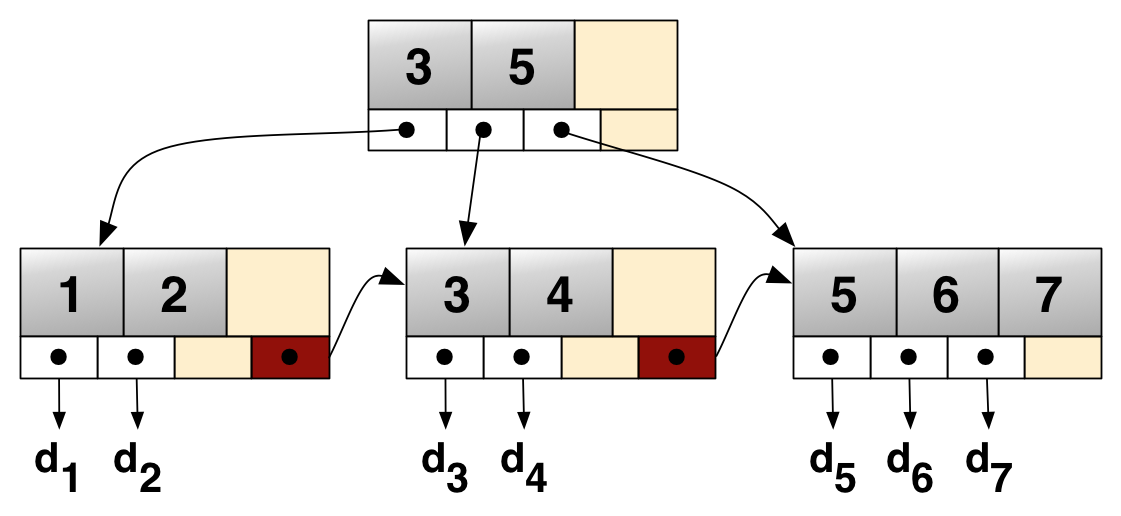
\includegraphics[width=10cm]{Bplustree}
\caption{Diagrama de uma árvore B+. Os números de 1 a 7 são chaves, e os dados armazenados na árvore estão identificados de $d_{1}$ a $d_{7}$.}
\label{bplustree}
\end{figure}

